%!TEX root = ../MasterThesis.tex

\section{Existing System Design Approaches}
\label{sec:system_approaches}

When trying to solve issues of information integration between organizations there are already existing solutions, that have to be examined whether they might fit the \gls{E-commerce} fraud investigation scenario or not.

\subsection{The \gls{ETL} processes}
\label{subsec:etl_process}

To begin with, retrieving, transforming and combining data from multiple dispersed data sources is not a completely new problem, and is actually part of ``Extract-Transform-Load'' or \gls{ETL} processes \textbf{\underline{within}} an organization. The basic idea is the same as in the concept shown in this thesis; namely to get as much information as possible from the various databases, that are in use within a company, harmonize (aka transform) the information from each of them into a shared data model, and use the cleaned up and combined information repository for doing advanced business analytics and predictions. Data within an organization is created and maintained by different business-related tools. Each of these will store the information into their own database using a vendor-specific schema. Other business-relevant data might be stored in structured files sometimes using a proprietary format, such as Excel files. Each of these data sources have to be accessed, the valuable information have to be extracted and mapped against each other, before the analysis of it can begin on a separate data store, that holds the combined data set. The whole process is visualized in Figure~\ref{fig:images_etl_process}. \\

\begin{figure}[!ht]
  \centering
  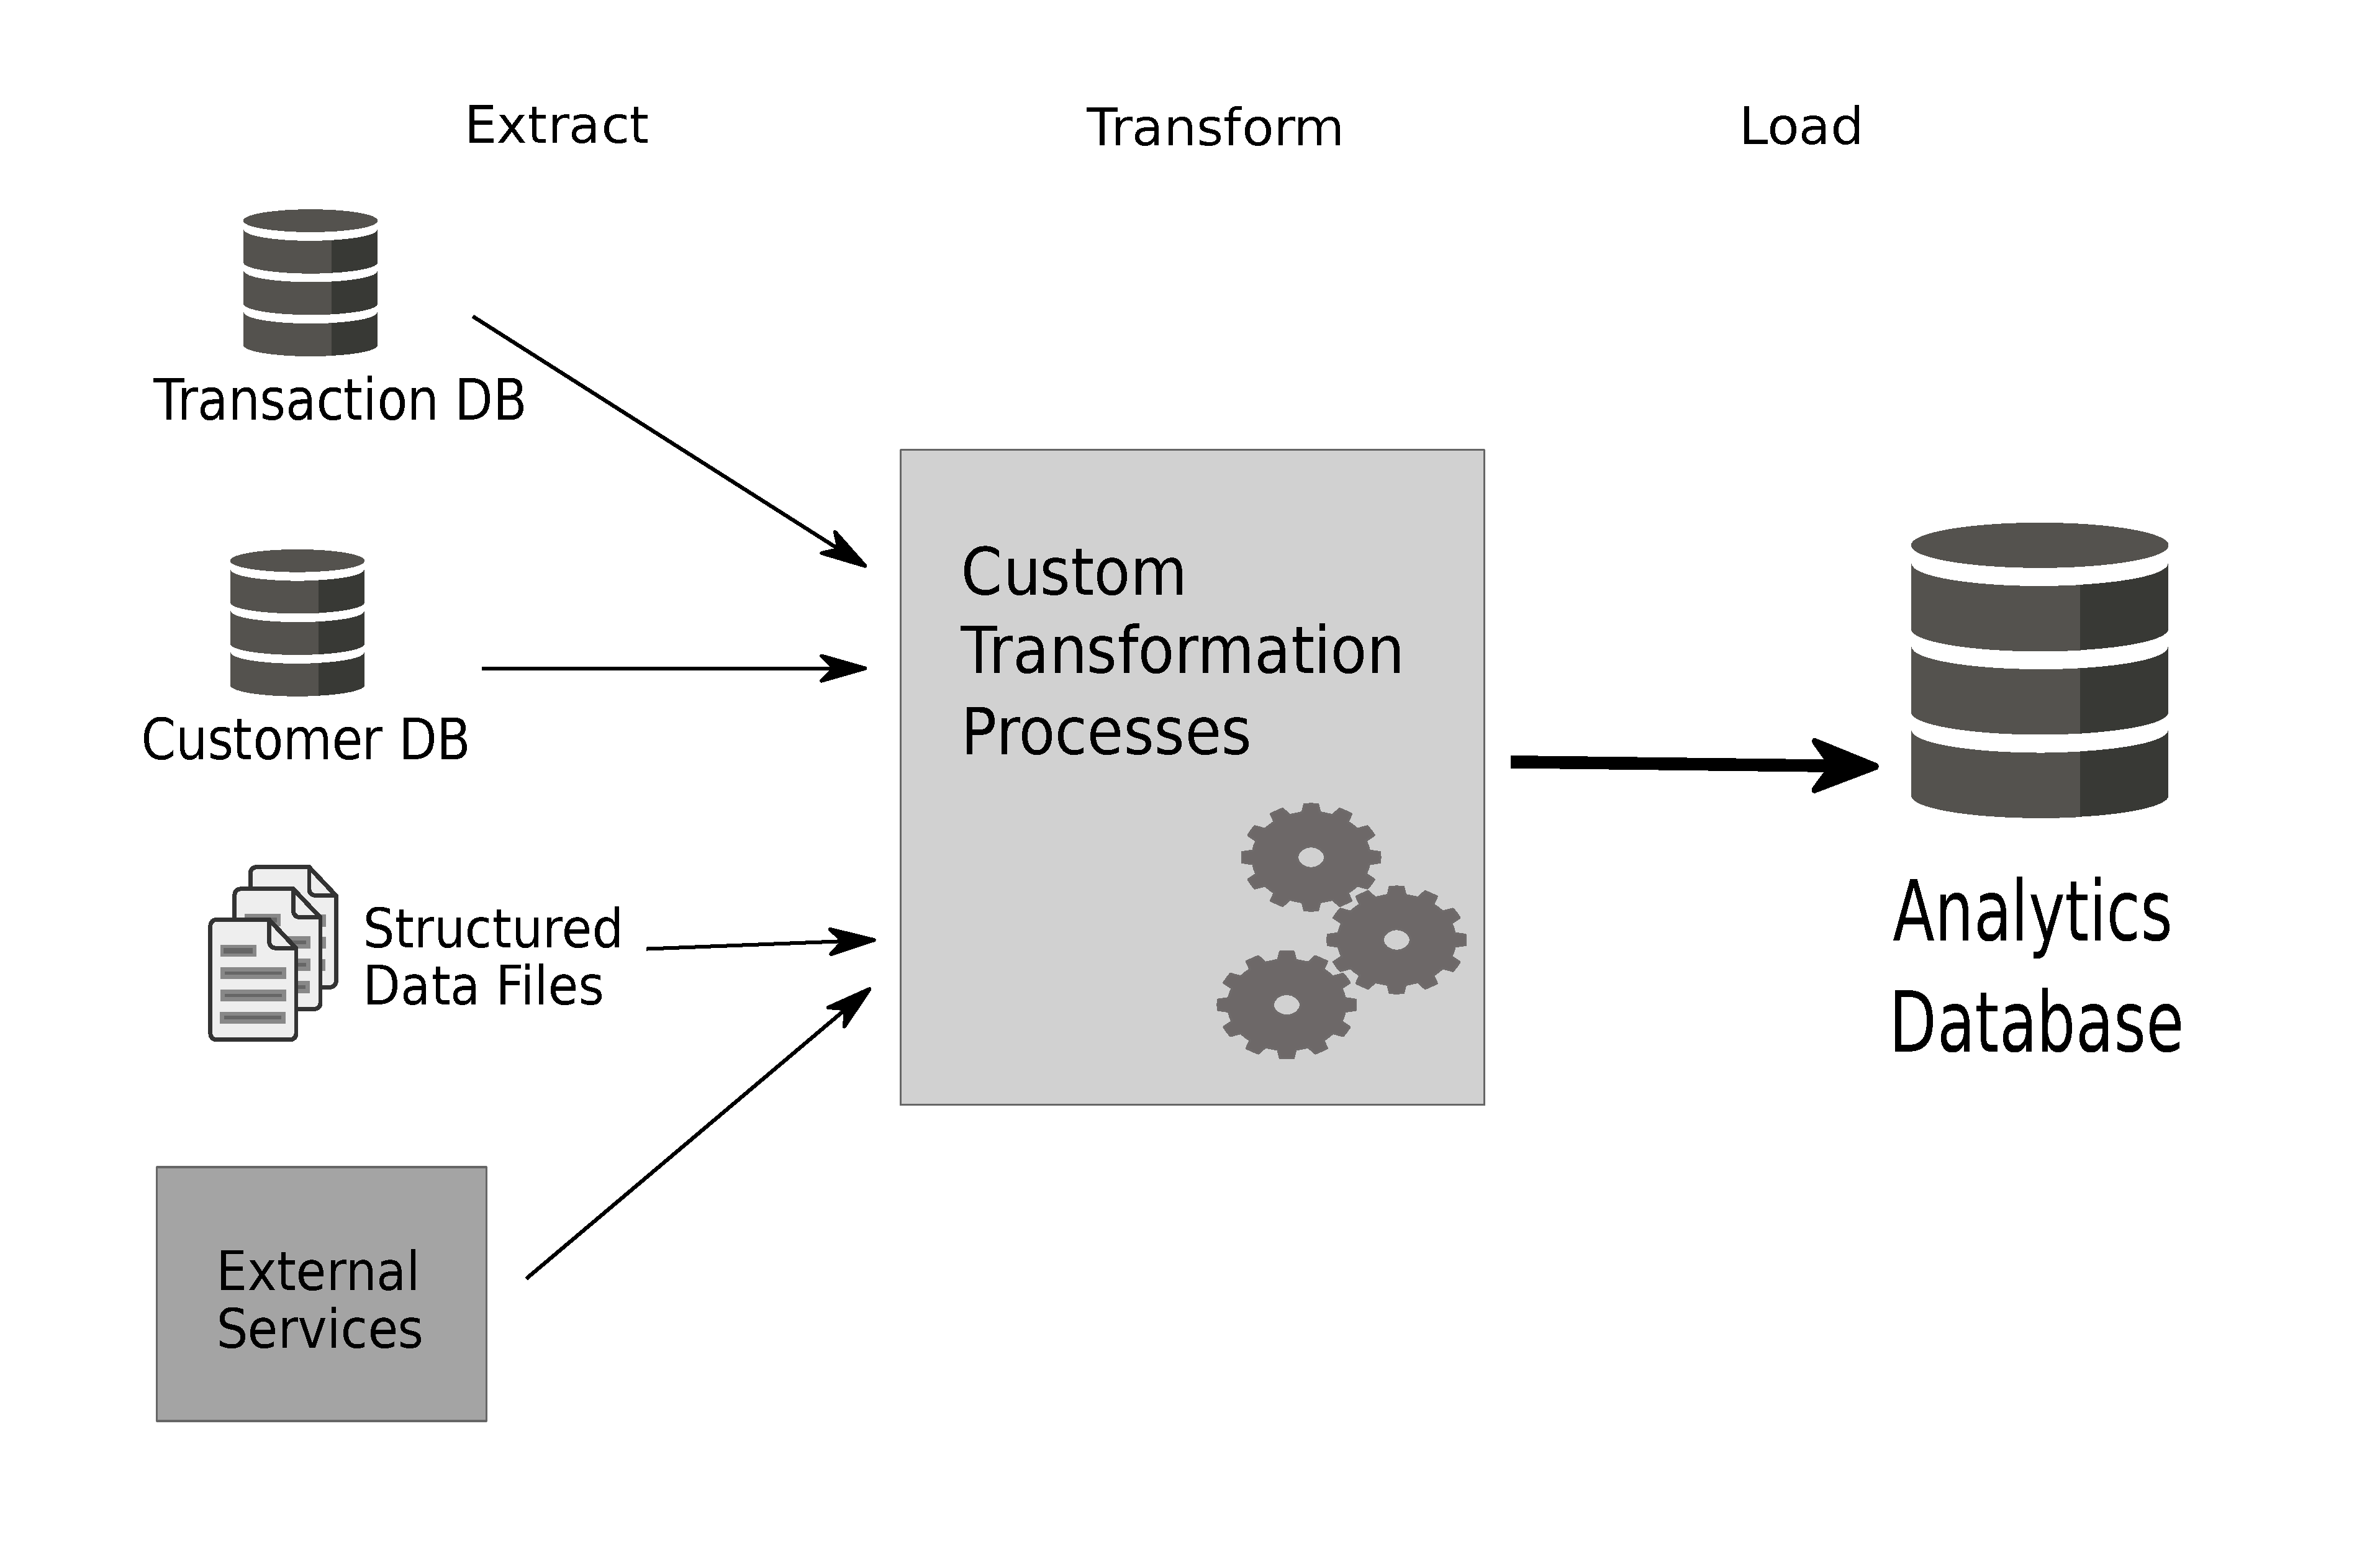
\includegraphics[width=0.9\columnwidth]{images/etl_process.pdf}
  \caption[ETL process within a company]{\gls{ETL} process within a company \citep[pg. 165]{wood2014linked}}
\label{fig:images_etl_process}
\end{figure}

Still these \gls{ETL} processes rely on an in-depth knowledge of the data structures, that are used in each of the information sources as well as require a direct access to the databases and files for retrieving the information. Although these conditions are not cumbersome to work with within an organization, they will be a real show stopper if one has to integrate data sources across company boundaries. As the integration of the information takes place on the database level, allowing external access to your internal databases will not only open up access to your business internals, but will also make it much more complicated to change the underlying database structures and business-related software tools in use. Any changes to one of these require an elaborate negotiation between the owner of the data source and all of the external partners attached to it. \\

Beside this obviously unsuitable application for the \gls{E-commerce} fraud investigation scenario at the whole, one can assume that these \gls{ETL} processes are still in use for operating the daily business of each stakeholder. They can be helpful at a later point in the discussion, when a decision has to be made about how a stakeholder can prepare and transform his internal data sources for external consumptions.

% section etl_process

\subsection{Web Services}
\label{subsec:web_services}

With the development of the \gls{E-commerce} scenario there was also a need to integrate business functionalities from various service providers, whose are operating on the Internet. Valid examples for this kind of integration are the usage of the \gls{PSP} for doing the payment as well as the \gls{LSP} for handling the shipping process. These approaches resulted in the ``Service Oriented Architecture'' paradigm, that enables application services provided by different vendors to talk to each other via a public facing programming interface (aka \gls{API}). The only requirement for such interoperability to work properly is, that each public interface follows some standardized or commonly agreed upon guidelines to be vendor-, platform- as well as language-agnostic. One possible implementation of these concepts are the so-called Web Services, that use the WS* protocols and standards from the \gls{W3C} with the extensible markup language (aka \gls{XML}) and the \gls{HTTP} protocol at their core \citep{josuttis2007soa}. \\

Like the \gls{HTML} format, that is used to represent Web pages on the Internet, \gls{XML} is originally based on \gls{SGML}, but instead of formalizing markup tags for structuring and styling textual content it is a meta-language allowing everyone to define his or her own markup languages. In this matter it doesn’t dictate what tags are available to structure the information; instead it includes some basic guidelines for creating well-formed and valid documents that uses domain-specific tags, which can be freely defined and structured by the creator of the \gls{XML} document. Therefore it is better suited in situations, in which a computer has to parse and evaluate the content of a message; assuming the computer program knows the structure of the message. \\

In an additional step the author of the \gls{API} could also specify an \gls{XML} schema for each message, which describes the structure of the message with all the possible elements, their ordering, nesting level and data types in detail. By doing so the \gls{XML} parser program can later verify the content of a retrieved message against the \gls{XML} schema and check if it is a valid document related to the schema definition. \gls{XML} schemata are also expressed in \gls{XML} format and have been standardized by the \gls{W3C}. Being able to create custom markup languages via \gls{XML} has a huge benefit for machine-to-machine communication and is the basis for integrating Web Services (via the WS* protocols), but it still has limitations when it comes to figure out the semantics of those \gls{XML} messages. This is mostly due to the fact that each \gls{XML} document represents a new markup language and needs a specific \gls{XML} parser to be understood by the machine; also to distinguish commonly used tag names in an \gls{XML} document the creator has to place them into specific namespaces (aka \gls{XML} namespaces). But those \gls{XML} namespaces further complicate the automatic processing of \gls{XML} documents and increases the necessity to have custom instances of \gls{XML} parsers for each \gls{XML} document \citep{taylor2008p2p}. \\

An integration of information exchange via Web Services is usually handled separately for each Web Service interface. Looking at the payment service integration as \textbf{\underline{one}} possible example, the following steps are necessary to allow a merchant to interact with the Web Service of a \gls{PSP}: \@

\begin{itemize}
  \item the \gls{PSP} has to define and implement an interface (aka \gls{API}) that a merchant can use to exchange information with them
  \item the \gls{API} includes a set of data exchange messages, usually in \gls{XML} format, as well as a list of operations, that the interface supports
  \item the \gls{PSP} has to document each of these messages and operations, incl.\ their intended structures and semantics
  \item the \gls{PSP} has to provide access to the \gls{API} via an \gls{HTTP} endpoint running on a server at a specific \gls{URL}
  \item the \gls{PSP} usually restricts access to this interface for registered partners only; for this they have to provide a registration and identification mechanism
  \item the merchant has to register with the \gls{PSP} to be able to call into their Web Service \gls{API}
  \item the merchant receives some kind of token, that they can use to identify themselves with the Web Service later
  \item the merchant has to implement an \gls{API}-specific client-side wrapper, that knows how to talk to the interface; incl.\ calling one of the available operations as well as serializing and deserializing the messages that will be transmitted between the Web Service and the client program
  \item the client program has to understand the structure and semantic of the messages exchanged with the Web Service
\end{itemize}

Although other merchants, that want to use the same \gls{API} from the \gls{PSP}, can use the same client-side wrapper (sometimes also provided by the \gls{PSP} for convenience) to send/receive messages to/from this specific Web Service, they still have to make the \gls{API}-specific integration into their own Web shop. Also, the integration is only done in an one-way direction. To allow the merchant to provide information from their own databases, the merchant has to do likewise and provide an \gls{API} for others to use to query for information (following the same steps as mentioned above). \\

Also, as the structures and semantics of the messages and operations of each Web Service interface are not standardized, integrating with another \gls{PSP} or merchant results in doing the same integration steps again and again. To make things worse, the mapping of the information coming from different \gls{API}s has to be implemented by the client, who wants to analyze the combined data set.   It soon becomes clear, that these necessary tasks will increase the time and effort with each additional stakeholder, who wants to participate in the collaborative system, see Figure~\ref{fig:web_services_scenario}. \@

\begin{figure}[H]
  \centering
  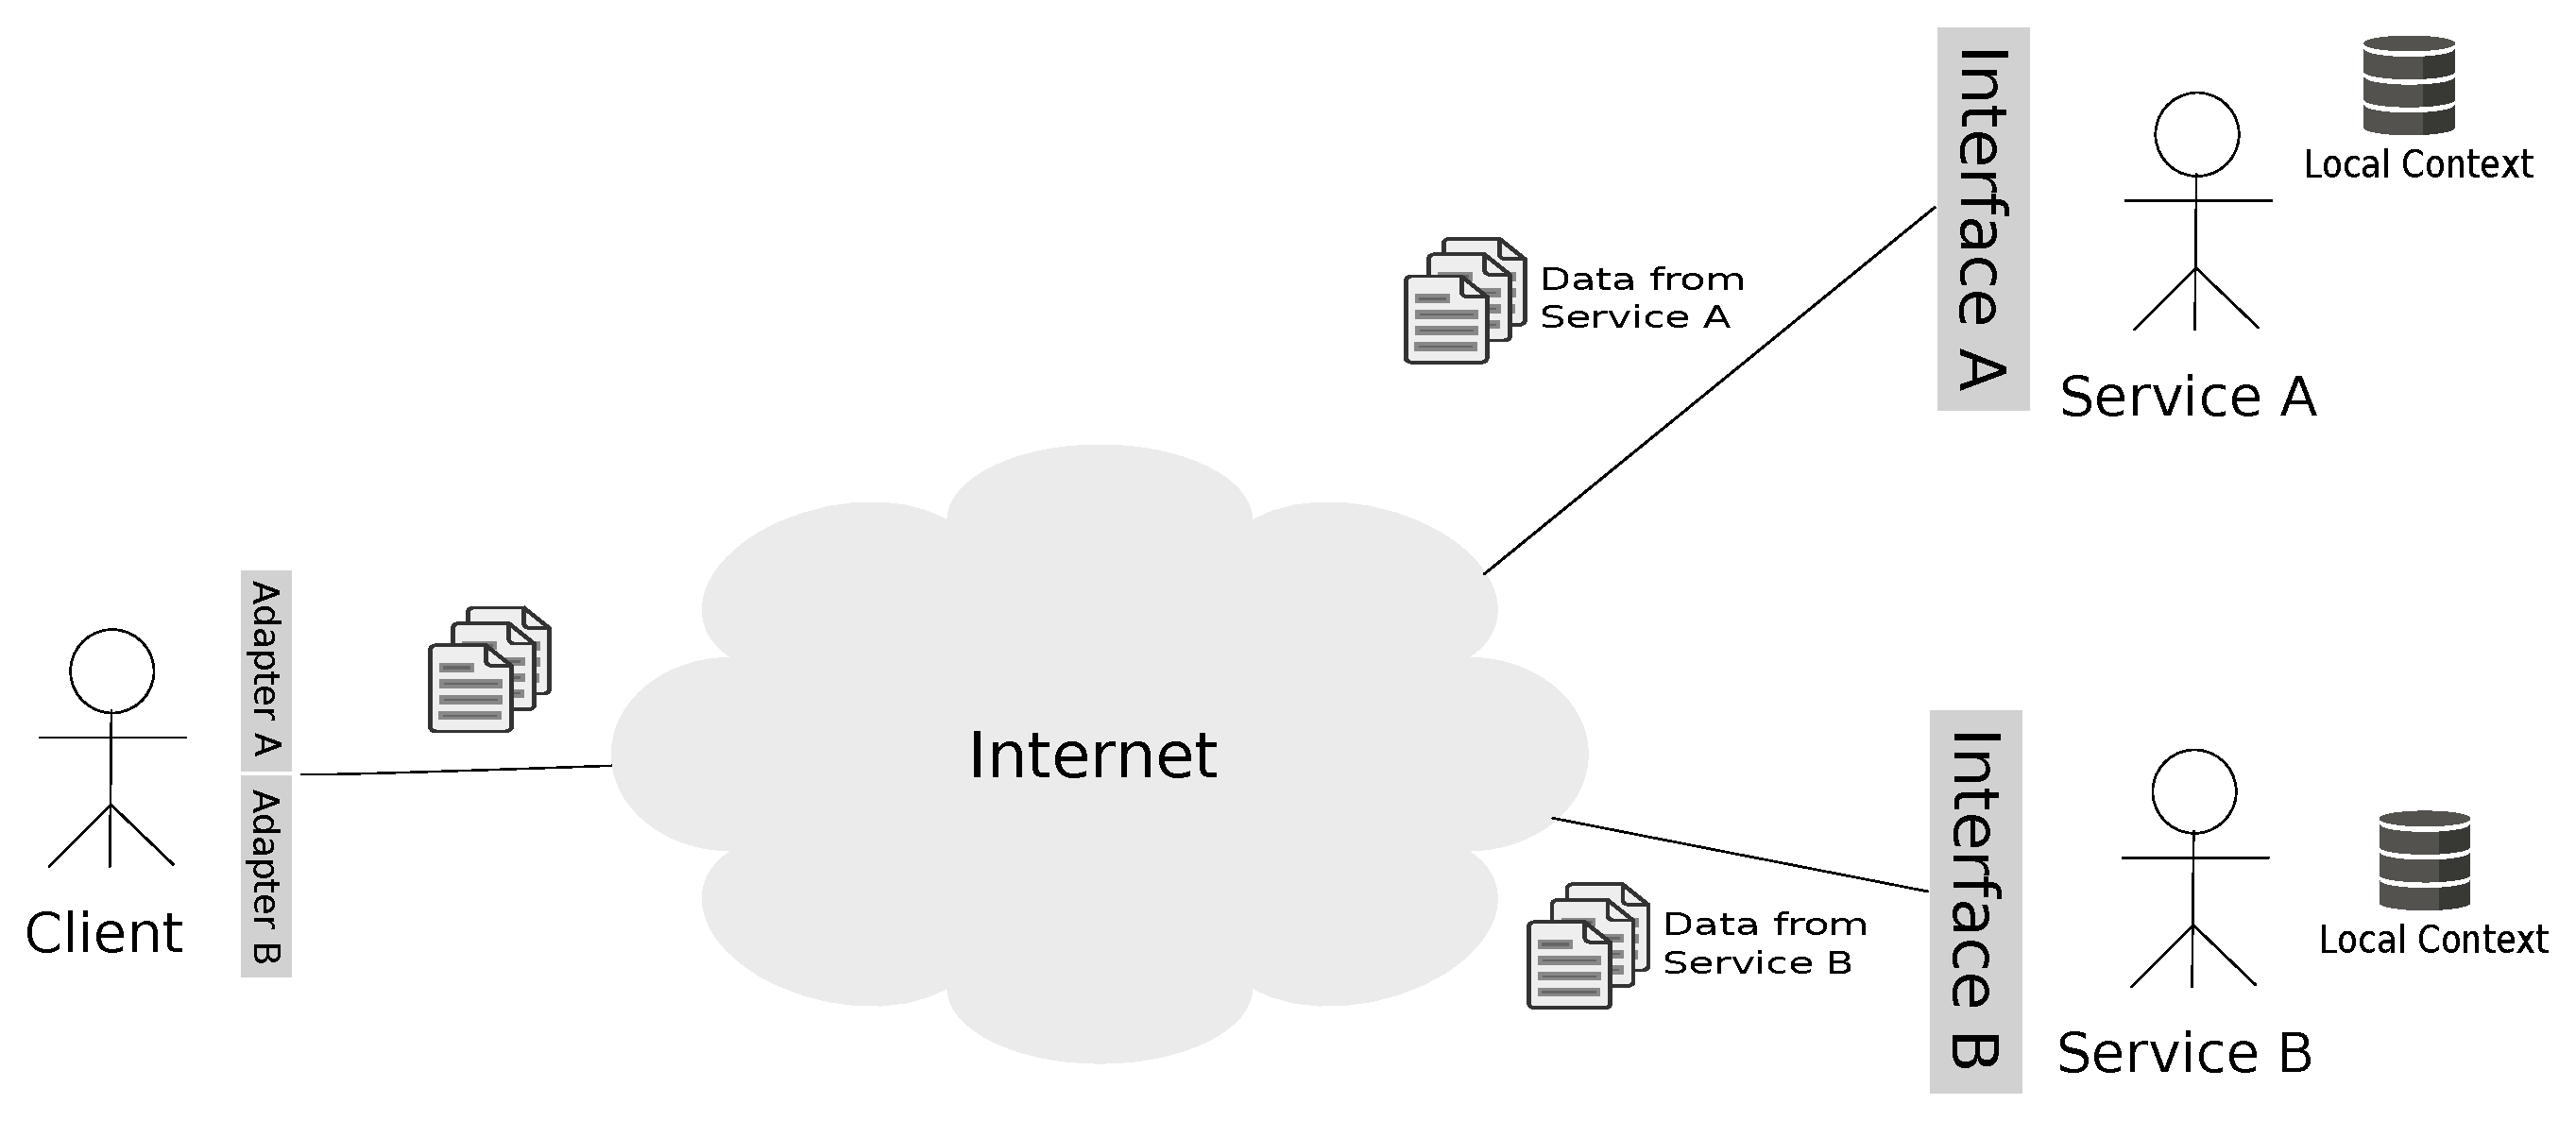
\includegraphics[width=0.9\columnwidth]{images/web-services-scenario.pdf}
  \caption{The Web Services scenario}
\label{fig:web_services_scenario}
\end{figure}

As conclusion one could easily see that integrating information between a larger group of participants is very limited with the existing Web Services approach. The steps necessary for exchanging information result in huge efforts on all participating parties. As there is no common way to access and combine the information from each one of the participants, beside using the fundamental \gls{HTTP} protocol and \gls{XML} data format, there have to be a lot of collaborative work between each of them upfront, to come up with an approach to integrate the available \gls{API}s, and provide the rules for combining the different data structures. Due to these restrictions one can assume that an integration based on the Web Services approach will only work with a limited number of participants. This might lead to a collaborative system, that will only include larger online retailers as participants, and therefore left out smaller shops from the \gls{E-commerce} fraud investigation process. For a solution of the problem described in Section~\ref{sec:scope_thesis} this is not sufficient. One need technologies that provide a better scalability and integration ability for the exchange of information between various, otherwise not strongly related organizations.

% subsection web_services (end)

\subsection{Semantic Web}
\label{subsec:web_data}

``The Web is full of intelligent applications, with new innovations coming every day'' \citep{allemang2011semantic}. But each of those intelligent Web applications is driven by the data available to them. Data that is likely coming from different places in the global information space — accessible usually via a custom API on the server hosting those resources (see Section~\ref{subsec:web_services}). The more consistent the data available to the smart Web application is, the better the Web service and its result will be. But to support an integration of the data from various Web services the semantics of the information delivered by each service has to be available — and there has to be a generalized, formalized way to express the semantic of that data. The focus on a standard that allows Web services to express the semantics of the data they provide also allows for global scalability, openness and decentralization, which are the key principles of the World-Wide Web. The Semantic Web tries to give a solution for this problem by providing the Resource Description Framework (aka \gls{RDF}) and related technologies (e.g. RDF schema, \gls{SPARQL}, \gls{OWL}, \ldots) for describing, linking and querying the data that a Web service delivers. But it doesn’t reinvent the wheel; instead the Semantic Web builds upon existing, proven technologies like \gls{XML}, XML namespaces, XML schemata and the \gls{URI} to uniquely address resources on the Web \citep{allemang2011semantic}. \\

The main benefits of the Semantic Web approach are the specification of a standardized and generalized format to exchange information on the Web (aka \gls{RDF}) as well as a commonly agreed way to access and query for them (aka \gls{SPARQL}). The \gls{RDF} data format does not only specify the syntax of the information exchanged, but also include the semantic (aka meaning) of them. Due to this fact, resources described in \gls{RDF} format are consistent and semantically self-contained. These characteristics are achieved by providing information as a ``triple''; that is a statement consisting of the resource in question (aka subject), a predicate and the specific value (aka object) for it. To be able to unambiguously identify the meaning of these statements, each part of them are usually expressed by utilizing unique \gls{URI}s. These \gls{URI}s can be abbreviated via ``prefix'' definitions to make the whole statement easier to read (see also Section~\ref{sec:semantic_web}). To specify that there is an order ``12345'' from ``merchant1'', one can come up with the following statement, that uses the explicit Schema.org specification \citep{Schema.org} to describe an order: \@

\begin{listing}[H]
  \inputminted[linenos,
               numbersep=5pt,
               breaklines=true,
               frame=lines]{TURTLE}
               {./samples/sample_order_12345.ttl}
  \caption{An order specification in \gls{RDF}}
\label{lst:sample_order_ttl}
\end{listing}

An \gls{RDF} file can contain one or more of such ``triples'' describing the resources of interest in detail. Usually these ``triples'' are visualized as directed graph, in that subjects and objects are displayed as nodes and predicates as edges between them. The above Listing~\ref{lst:sample_order_ttl} can be presented as graph like this:\@

\begin{figure}[H]
  \centering
  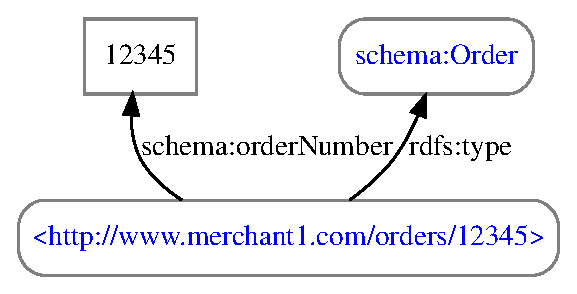
\includegraphics[width=0.8\columnwidth]{images/sample_order_12345.pdf}
  \caption{Graph-based visualization of \gls{RDF} from Listing~\ref{lst:sample_order_ttl}}
\label{fig:sample_order_graph_image}
\end{figure}

Beside having to provide internal resources in an understandable \gls{RDF} format the Semantic Web also specifies how to query and access the ``information databases'' on the Web. For this purpose the \gls{SPARQL} language and protocol is used. It does not only describe a query language, but also shows how to setup an \gls{HTTP} endpoint on a server to make the data set publicly available on the Internet. \\

Based on the specifications of the Semantic Web standards each relevant participant of an \gls{E-commerce} fraud investigation system will have to transform the information from their internal databases into a set of ``triples'' with commonly agreed upon \gls{URI} references. These additional data sets will be made available publicly on the Web for information retrieval via the \gls{SPARQL} language and protocol. Each participant of the collaborative system just needs to know the specific addresses of the \gls{SPARQL} endpoints to be able to query them for information. The results of each query can be easily combined into a new data set based on the merging capabilities of the \gls{RDF} standard. This will decrease the efforts for integrating the data from various external sources drastically. Also communicating with the different \gls{HTTP} endpoints to access and query for information is being done in a much more efficient way based on the \gls{SPARQL} protocol, see Figure~\ref{fig:web_data_scenario}. \@

\begin{figure}[H]
  \centering
  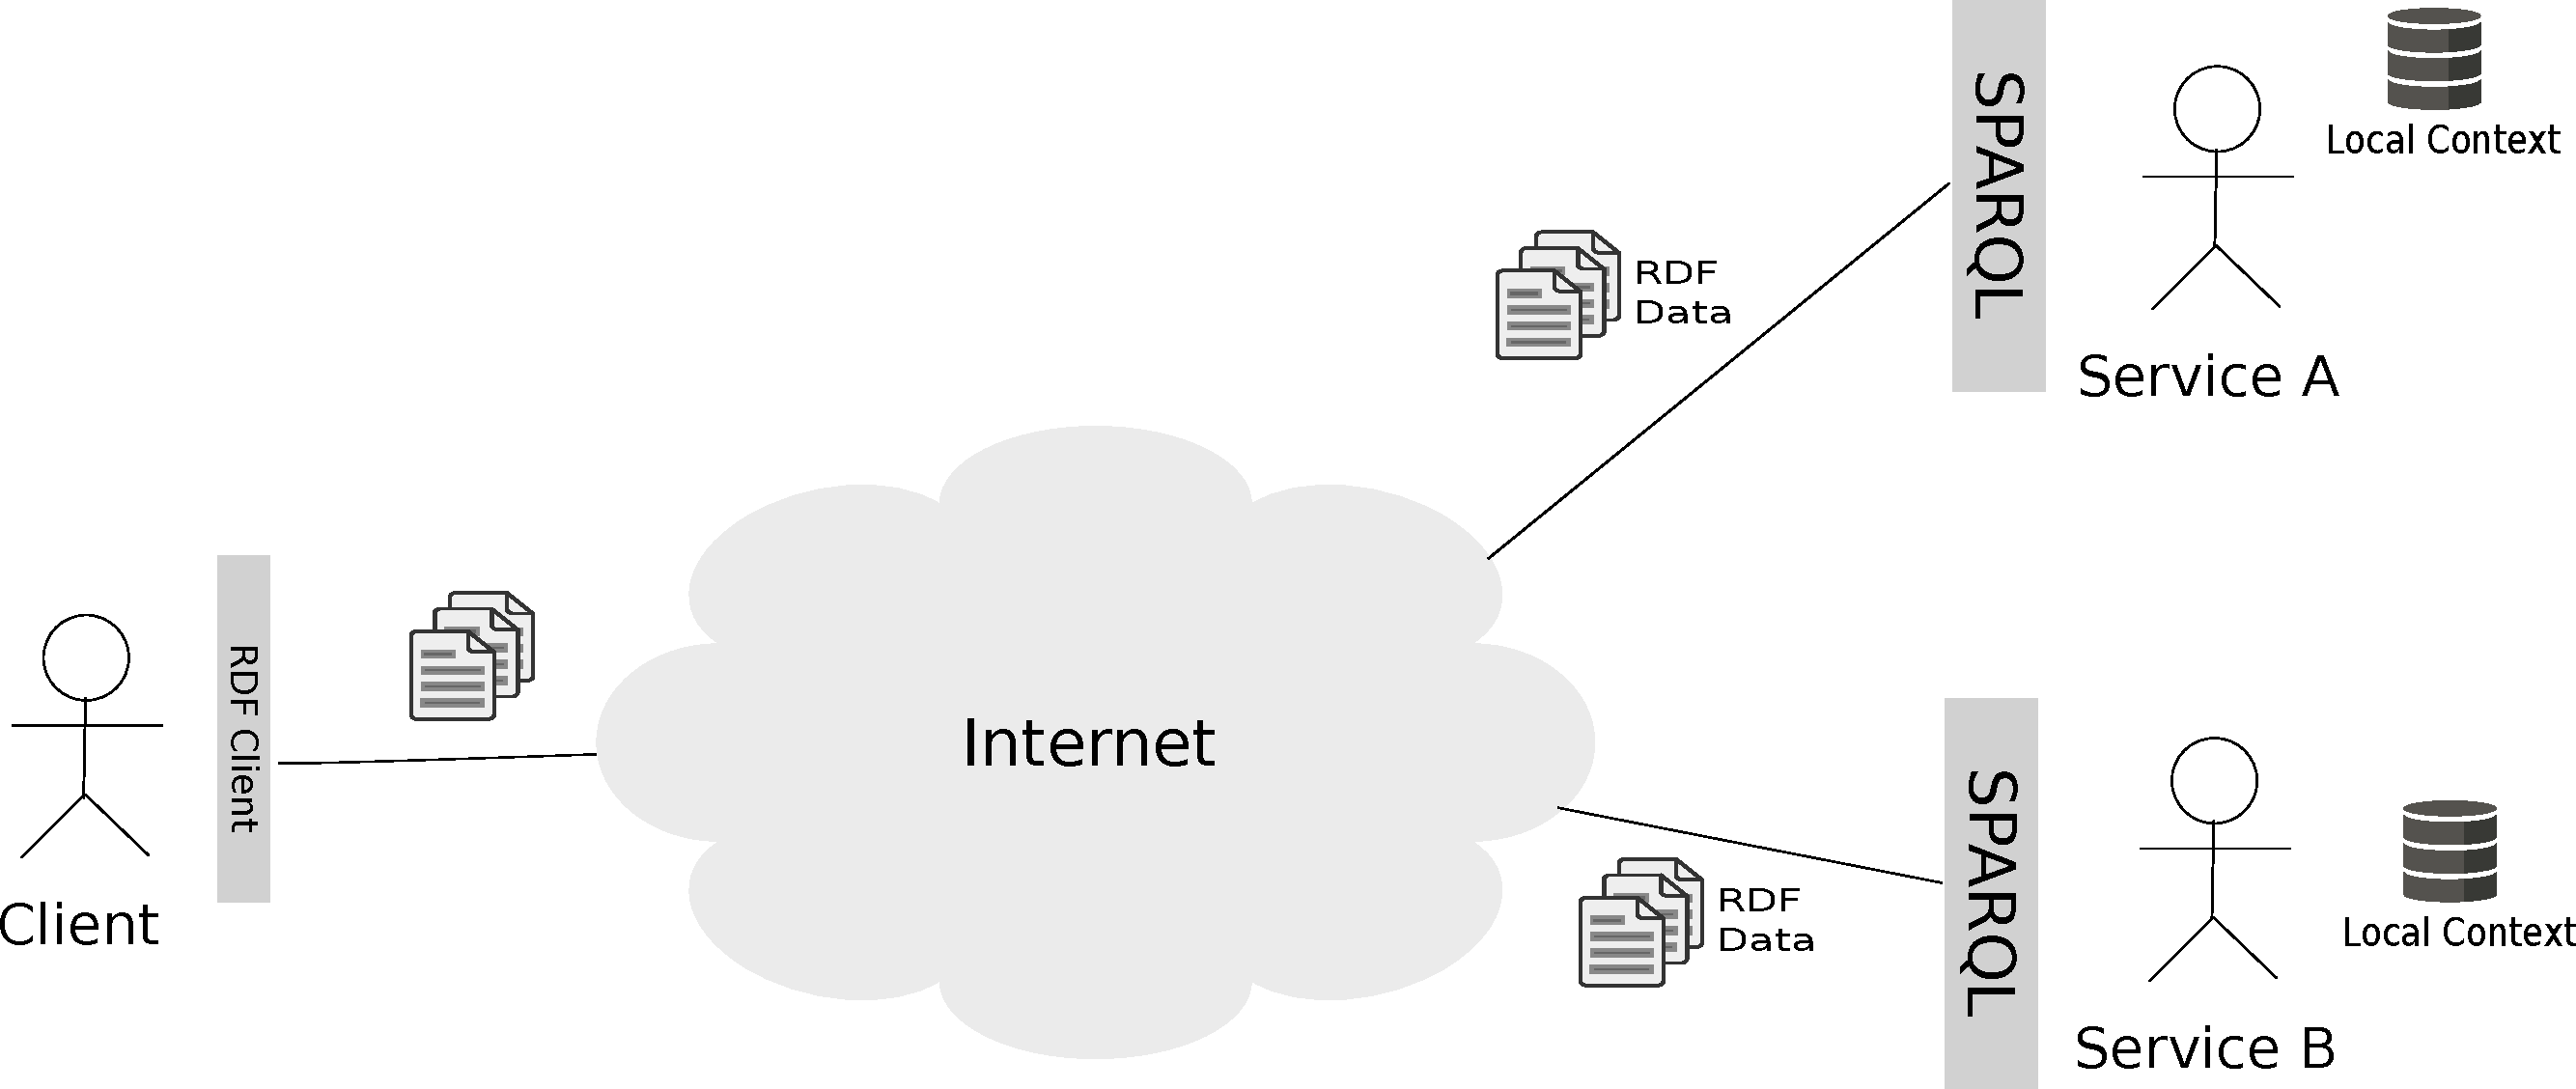
\includegraphics[width=0.9\columnwidth]{images/web-data-scenario.pdf}
  \caption{The Semantic Web scenario}
\label{fig:web_data_scenario}
\end{figure}

As the underlying model of an \gls{RDF} data set is resembling a graph-based representation it will fit the concept of the proposed system from Section~\ref{sec:design_proposal} perfectly. Still requiring any participant to setup and operate a public available \gls{SPARQL} server will limit the use of this architecture for the solution of the \gls{E-commerce} fraud investigation scenario. As parts of the information, that have to be exchanged between the relevant participants are confidential and/or business-critical to them, requiring a public \gls{HTTP} endpoint on the Internet, is a high security risk. Additionally the \gls{SPARQL} language and protocol does not offer a way to restrict access to only a subset of the information in the \gls{RDF} data store. Any party, who is aware of the \gls{URL} of the \gls{SPARQL} endpoint have access to all the information, that are in the underlying \gls{RDF} data stores (see Listing~\ref{lst:get_them_all_sparql}). It is therefore no surprise, that there are currently only a small set of publicly available \gls{SPARQL} endpoints on the Internet --- with the most commonly used one from DBpedia.org \citep{dbPedia.org}, that is offering public available data from Wikipedia articles in \gls{RDF} format. \@

\begin{listing}[!ht]
  \inputminted[linenos,
               numbersep=5pt,
               breaklines=true,
               frame=lines]{SPARQL}
               {./samples/get_all_records.sparql}
  \caption{Retrieving all information in an \gls{RDF} store using \gls{SPARQL}}
\label{lst:get_them_all_sparql}
\end{listing}

To conclude, one can assert that the fundamental technologies of the Semantic Web standards are a good fit for exchanging and merging information between different stakeholders. But the usage of an all or nothing approach for querying the \gls{RDF} data stores via \gls{SPARQL} is way to open for the proposed solution.

% subsection web_data (end)

% section system_approaches (end)
